\chapter{Przebieg badań}
Doświadczenie polegało na analizie porównawczej sprawności algorytmów opisanych w \refsource{rozdziale}{cha:dos} w \refsource{sekcji}{sec:alg}. Celem doświadczenia było określenie jakości algorytmu utworzonego w ramach pracy inżynierskiej autora\cite{Blyszcz2022}. Szczegółowa metodologia badawcza została określona w \refsource{podrozdziale}{sec:met}.


\section{Metodologia badawcza}
\label{sec:met}
Przyjęta w projekcie metodologia badawcza została określona w poniższej \refsource{tabeli}{tab:met-bad}. Przyjęta metodologia ma za zadanie określić jakoś porównywanego algorytmu.

\begin{table}[H]
    \centering
    \captionsource{Metodologia badawcza}{Opracowanie własne}
    \begin{tabular}{|L{\textwidth}|}
        \hline
        \textbf{Problem badawczy:}                                                                                                                     \\
        Czy algorytm klasyfikacji danych utworzony w ramach pracy inżynierskiej może konkurować z rozwiązaniami dostępnymi w środowiskach komercyjnych \\ \hline

        \textbf{Pytania badawcze:}                                                                                                                     \\
        \begin{enumerate}
            \item Czy algorytm jest konkurencyjny pod względem wybranych metry:
            \begin{itemize}
                \item dokładność algorytmu
                \item czas działania
                \item precyzja
                \item czułość
                \item f1
                \item auc
            \end{itemize}
        \end{enumerate}                                                                                                                                \\ \hline

        \textbf{Hipotezy:}                                                                                                                             \\
        \begin{enumerate}
            \item Nie ma istotnej różnicy w wynikach próby testowej i treningowej.
            \item Nie ma istotnej różnicy w uzyskanej ''\textit{dokładności}'' między algorytmami.
            \item Nie ma istotnej różnicy w uzyskanej ''\textit{czułości}'' między algorytmami.
            \item Nie ma istotnej różnicy w uzyskanej ''\textit{precyzji}'' między algorytmami.
            \item Nie ma istotnej różnicy w uzyskanym ''\textit{auc}'' między algorytmami.
            \item Nie ma istotnej różnicy w uzyskanej ''\textit{f1}'' między algorytmami.
            \item Nie ma istotnej różnicy w uzyskanym ''\textit{czasie działania}'' między algorytmami.
        \end{enumerate}                                                                                                                                \\ \hline
    \end{tabular}
    \label{tab:met-bad}
\end{table}


\section{Przygotowanie platformy}
Do badań wykorzystano narzędzie ''\textit{Projektant}'' znajdujące się na platformie ''\textit{Azure Machine Learning Studio}'' (Azure ML). Narzędzie to umożliwiło utworzenie interaktywnego potoku zadań. Potok ten składa się z kilku części:
\begin{itemize}
    \item Przygotowanie i obróbka zbiorów danych
    \item Trenowanie oraz testowanie algorytmów klasyfikacji danych
    \item Utworzenie tabeli porównawczej dla wyników poszczególnych algorytmów (\refsource{obraz}{fig:pipeline}).
\end{itemize}

\subsection{Przygotowanie danych}
W pierwszym kroku dane zostały znormalizowane za pomocą metody \textbf{MinMax}, która przekształca dane numeryczne do wartości w zakresie ${0, 1}$. W następnym kroku za pomocą języka Python oraz biblioteką Pandas oraz Numpy zostają zamienione etykiety słowne na wartości \textbf{0} i \textbf{1} oraz następuje zamiana wartości $[NaN, -inf, inf]$ na cyfrę $0$. Cały proces został zobrazowany na \refsource{diagramie}{fig:norm}

\begin{figure}[H]
    \centering
    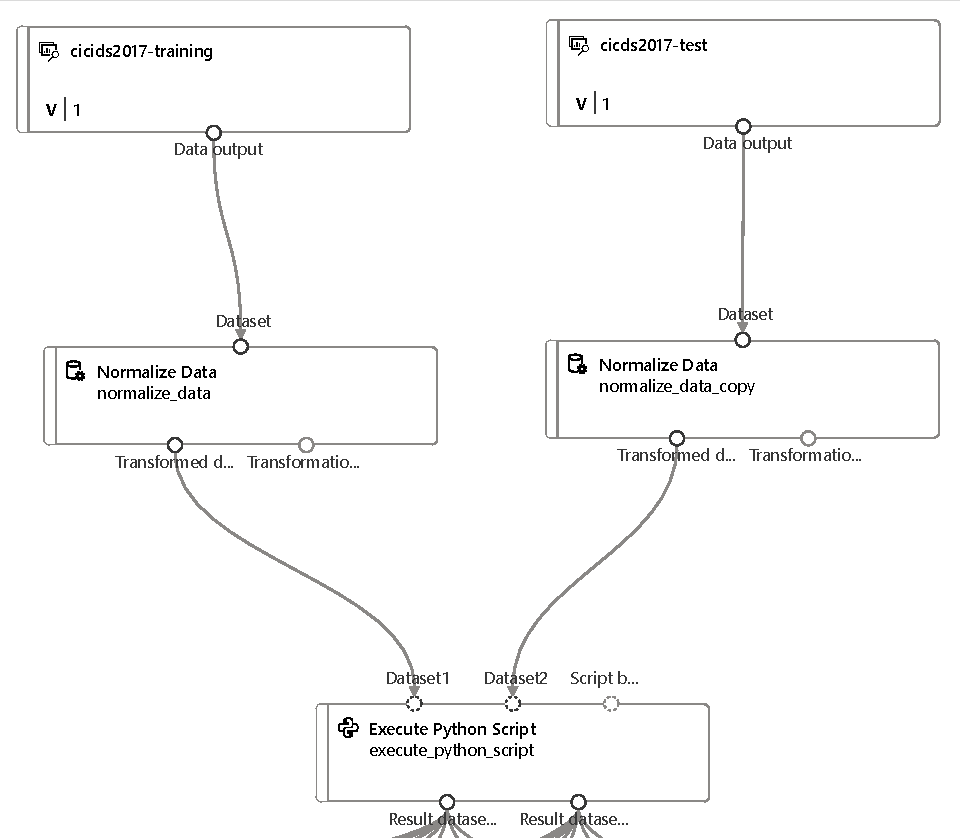
\includegraphics[width=0.6\textwidth]{images/norm}
    \captionsource{Potok normalizacji danych}{Opracowanie własne}
    \label{fig:norm}
\end{figure}

\subsection{Trenowanie oraz testowanie algorytmów}
Kolejną grupą zadań widoczną w potoku są te związane z trenowaniem i testowaniem poszczególnych algorytmów opisanych w \refsource{rozdziale}{cha:dos}. Każdy test składa się 3 kafelek. W przypadku algorytmów dostarczonych wraz z platformą Azure ML są to:
\begin{itemize}
    \item \textbf{model klasyfikujący} - odpowiada za przygotowanie algorytmu klasyfikacyjnego
    \item \textbf{blok treningowy} - tworzy wytrenowany model, za pomocą połączonego zbioru danych
    \item \textbf{blok ewaluacyjny} - sprawdza wcześniej wytrenowany model za pomocą powiązanego zbioru danych.
\end{itemize}
Potok zadań wykorzystujący algorytmy dostarczone przez Microsoft Azure został ukazany na \refsource{schemacie}{fig:ms-pipe}

\begin{figure}[H]
    \centering
    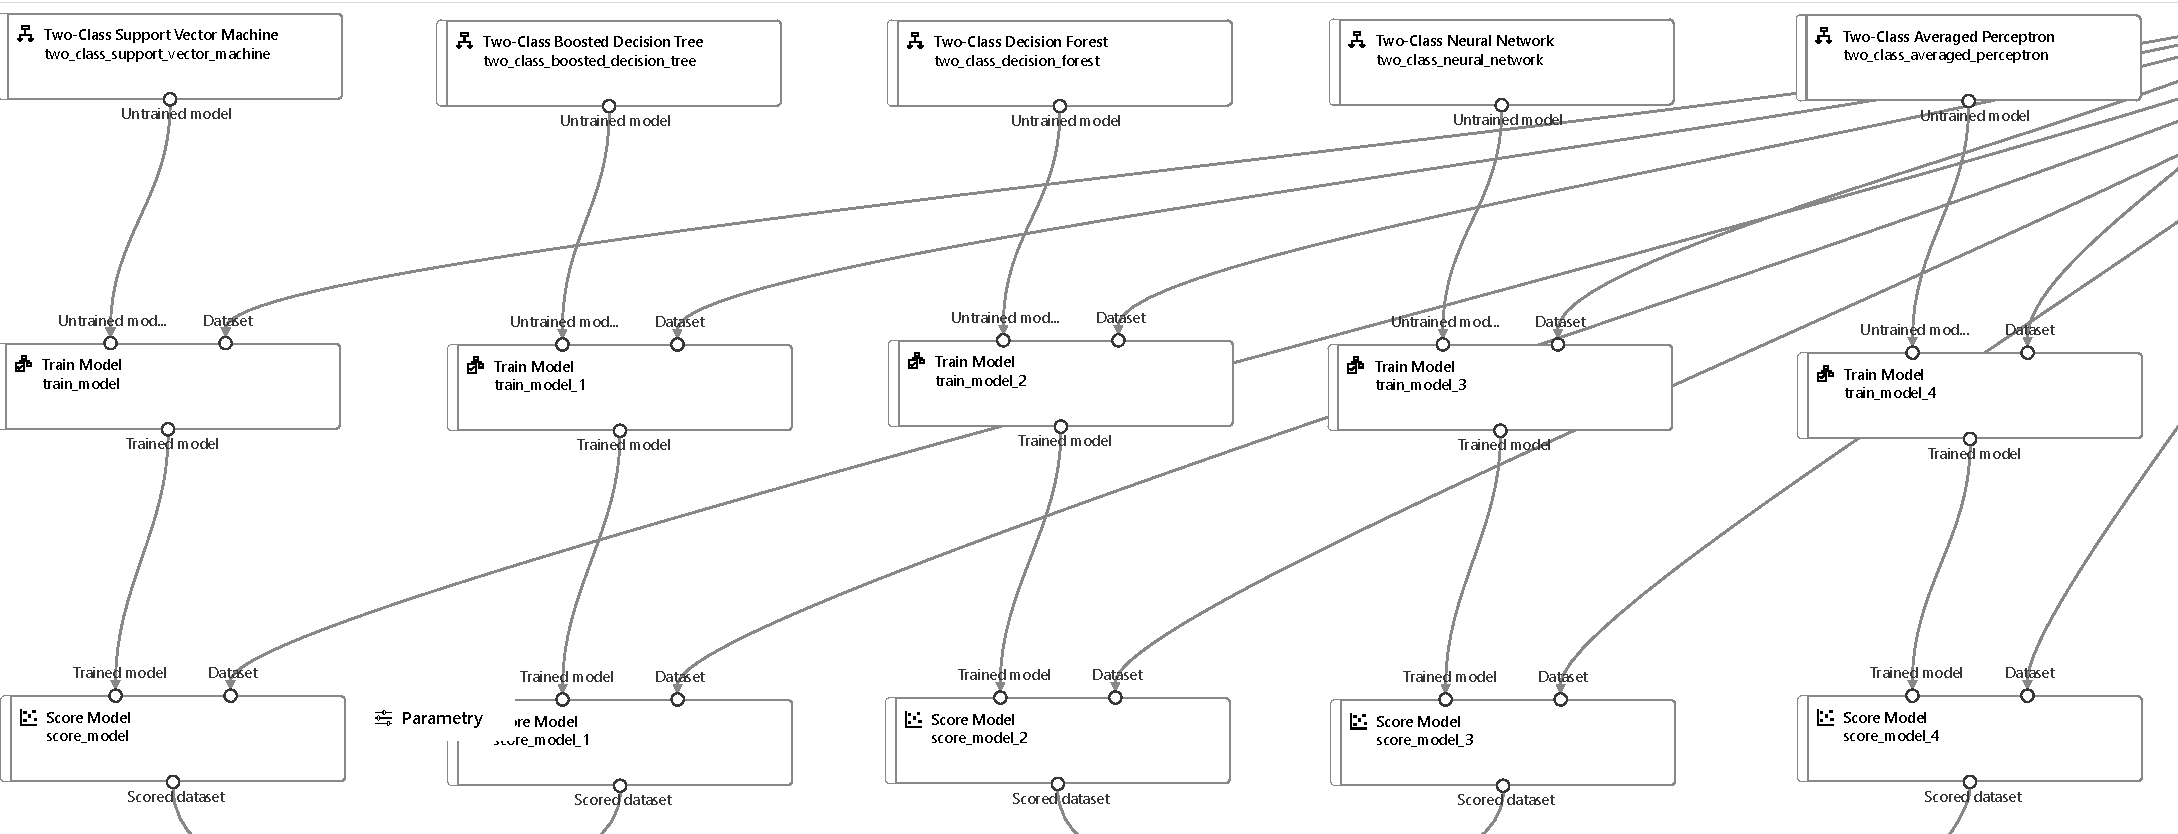
\includegraphics[width=\textwidth]{images/ms_pipe}
    \captionsource{Potok zadań dla algorytmów klasyfikacyjnych}{Opracowanie własne}
    \label{fig:ms-pipe}
\end{figure}

Algorytmy dostarczone w ramach pracy badawczej składają się z:
\begin{itemize}
    \item \textbf{biblioteka Python} - archiwum o rozszerzeniu \textbf{.zip}, które zawiera w sobie odpowiednie pliki napisane w języku Python
    \item \textbf{blok treningowy} - wykorzystuje dostarczoną bibliotekę do wytrenowania modelu oraz zapisania na platformie Azure najlepszego uzyskanego wyniku za pomocą powiązanego zbioru danych
    \item \textbf{blok ewaluacyjny} - wykorzystuje dostarczoną bibliotekę do ewaluacji algorytmu za pomocą połączonego zbioru danych
\end{itemize}

Potok zadań dla algorytmów niestandardowych został ukazany na \refsource{rysunku}{fig:au-pipe}

\begin{figure}[H]
    \centering
    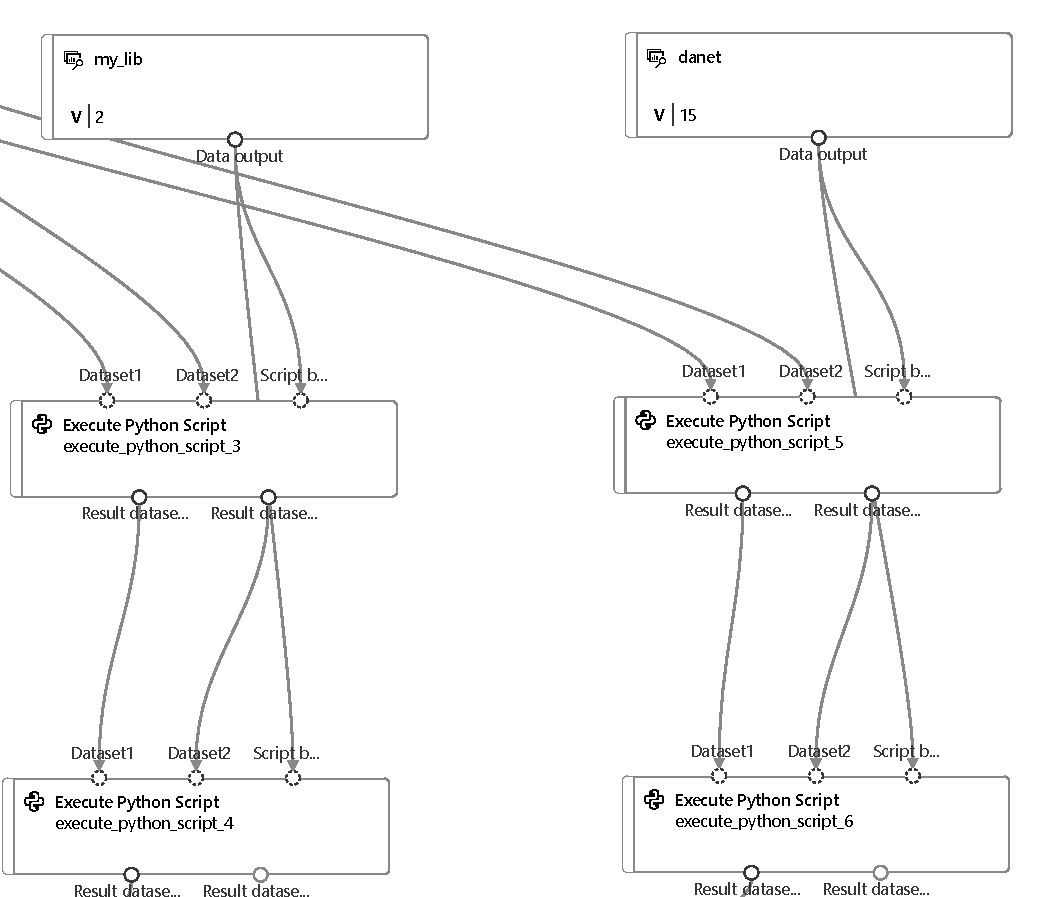
\includegraphics[width=0.8\textwidth]{images/au-pipe}
    \captionsource{Potok zadań dla algorytmów klasyfikacyjnych}{Opracowanie własne}
    \label{fig:au-pipe}
\end{figure}

\subsection{Utworzenie tabeli porównawczej}
Kolejną częścią zadań jest zebranie wyników poszczególnych algorytmów oraz połączenie ich w jedną całość. Wykorzystano do tego moduły języka Pyton, które zwracają przetwożone wyniki oraz łączą je w jedną tabelę zbiorczą, co pokazano na \refsource{rysunku}{fig:pipe-4}.

\begin{figure}[H]
    \centering
    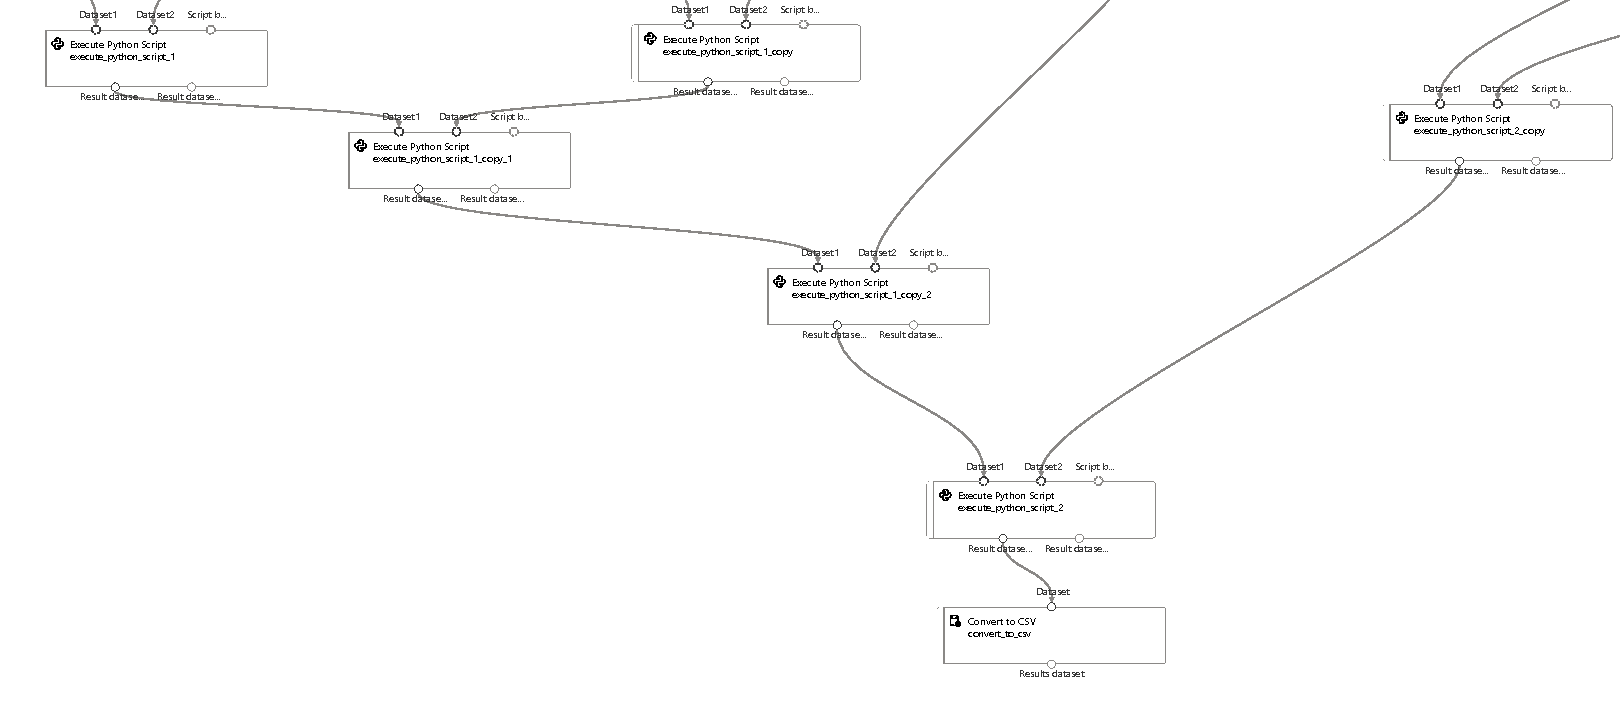
\includegraphics[width=\textwidth]{images/pipe-csv}
    \captionsource{Moduły odpowiedzialne za przetwożenie wyników}{Opracowanie własne}
    \label{fig:pipe-4}
\end{figure}


\section{Weryfikacja potoku}
Aby zweryfikować działanie całego procesu wykorzystano znormalizowane dane treningowe do wytrenowania oraz przetestowania działania algorytmów klasyfikacyjnych. Cały proces trwał ''\textbf{1 dzień 10 godzin 55 minut 53 sekundy}''. Wyniki tych działań widać na \refsource{rysunku}{fig:predict-same}. Analizując wykres można zauważyć, że uzyskane wyniki znajdują się w przedziale $[94\%, 100\%]$ w każdej metryce co pokazuje jakość każdego z algorytmów, a także to, że algorytmy poradziły sobie niemal bezbłędnie w rozpoznawaniu ruchu sieciowego, na którym były uczone. Zbiór, który wykorzystano do trenowania oraz testowania danych zawierał w sobie 225805 wpisów z czego 97718 należało do klasy ''\textbf{1}'', zaś 128087 należało do klasy ''\textbf{0}''.

\begin{table}[H]
    \centering
    \captionsource{Liczba elementów przynależących do danej klasy w zniorze treningowym}{Opracowanie własne}
    \label{tab:trening-data-label}
    \begin{tabular}{|c|r|}
        \hline
        \textbf{Klasa} & \textbf{Liczba wystąpień} \\ \hline
        1              & 97718                     \\ \hline
        0              & 128027                    \\ \hline
        \textbf{Suma}  & 225805                    \\ \hline
    \end{tabular}
\end{table}

Bazując na tym zbiorze oraz uzyskanych wynikach udało się udowodnić poprawność działania procesu klasyfikacji wieloma algorytmami genetycznymi.

\begin{landscape}
    \vspace*{\fill}
    \begin{figure}[H]
        \centering
        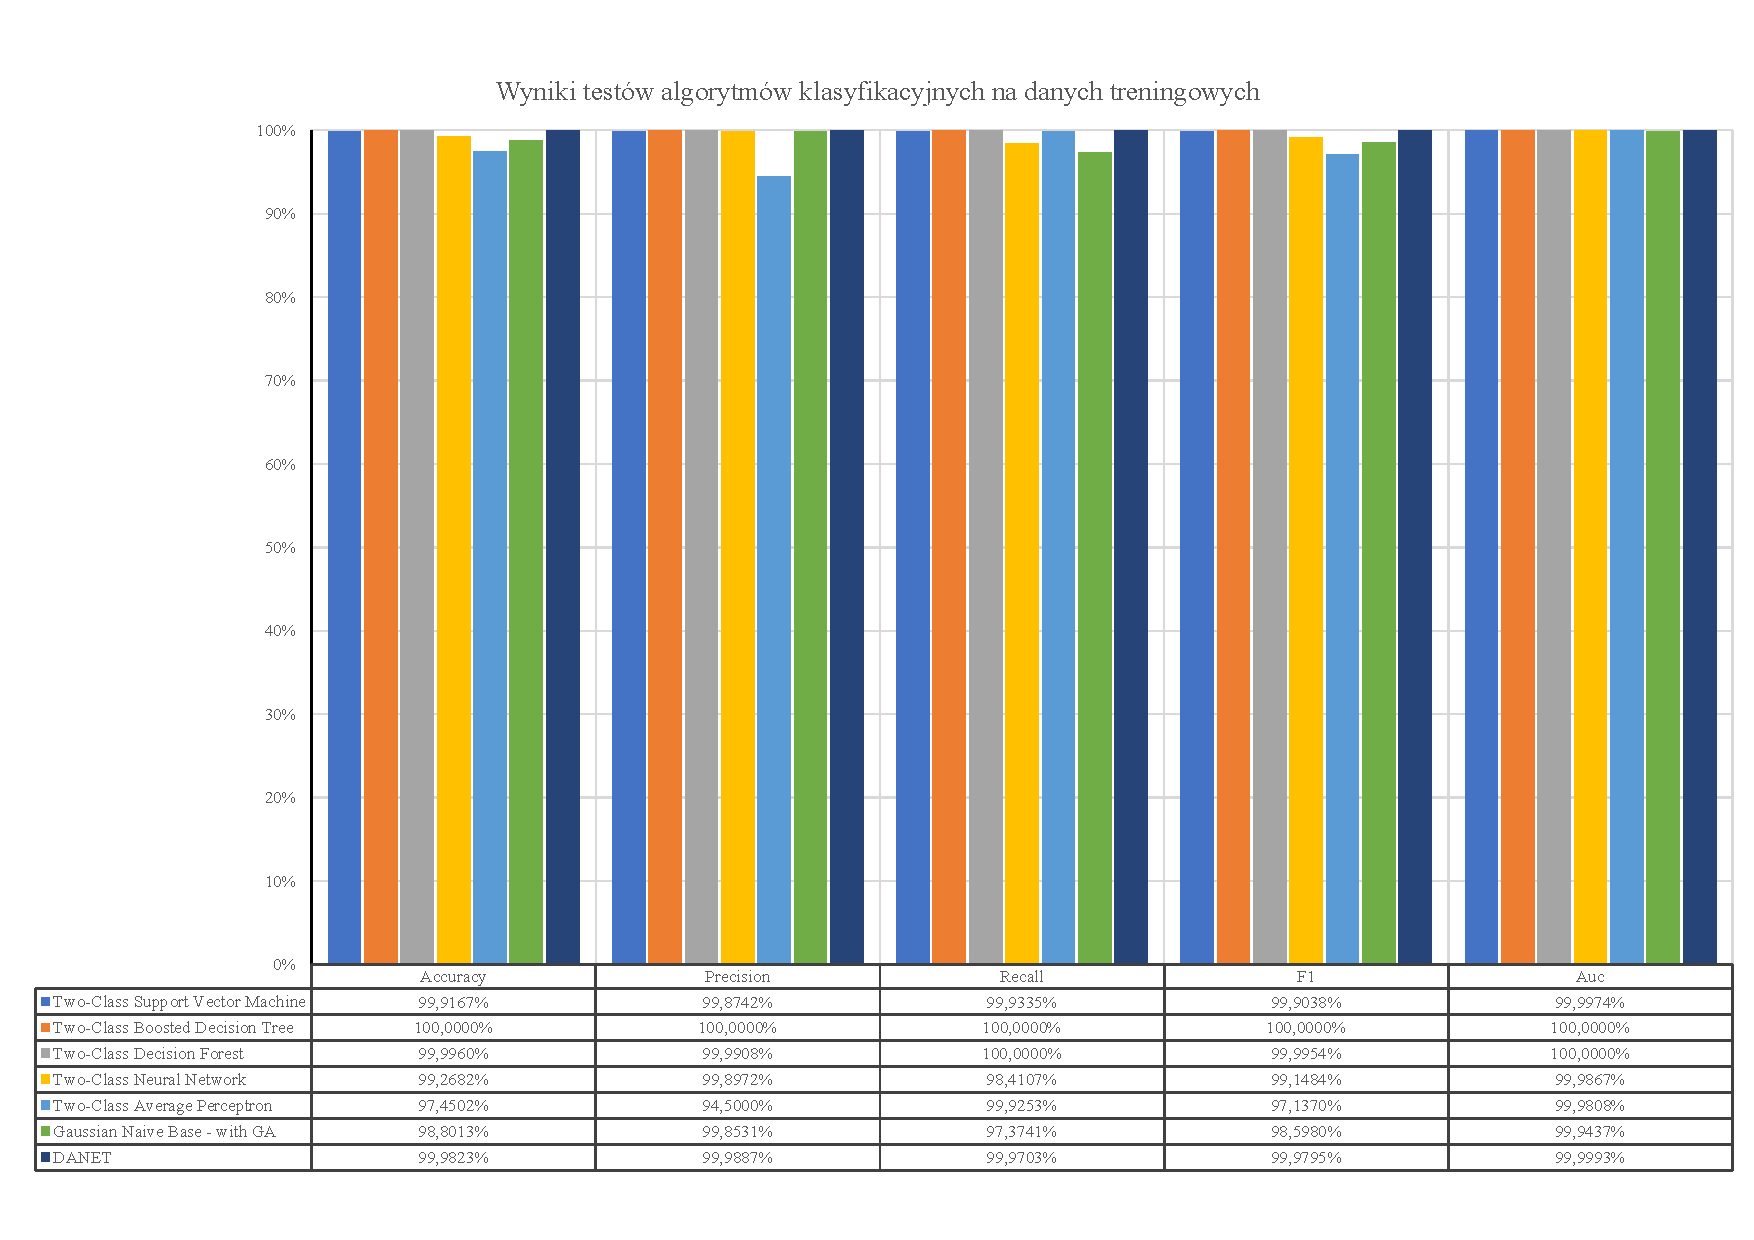
\includegraphics[height=0.8\textwidth]{images/predict_same}
        \captionsource{Wyniki testów algorytmów klasyfikacyjnych na danych treningowych}{Opracowanie własne}
        \label{fig:predict-same}
    \end{figure}
    \vfill
\end{landscape}


\section{Próba badawcza}
Aby uzyskać realne wyniki podczas porównywania poszczególnych algorytmów zastosowano zbiór treningowy opisany w \refsource{tabeli}{tab:trening-data-label} oraz zbiór testowy, który zawierał 2273097 wpisów należących do klasy ''\textbf{1}'' oraz 557646 wpisów należących do klasy ''\textbf{0}'' co sumarycznie daje: 2830743 wpisów tak jak to zostało pokazane w \refsource{tabel}{tab:res-test}.\ Pomiary testowe powtórzono 2 razy dzięki czemu uzyskano 3 próby badawcze.

\begin{table}[H]
    \centering
    \captionsource{Liczba elementów przynależących do danej klasy w zbiorze testowym}{Opracowanie własne}
    \label{tab:res-test}
    \begin{tabular}{|c|r|}
        \hline
        \textbf{Klasa} & \textbf{Liczba wystąpień} \\ \hline
        1              & 2273097                   \\ \hline
        0              & 557646                    \\ \hline
        \textbf{Suma}  & 2830743                   \\ \hline
    \end{tabular}
\end{table}

\begin{landscape}
    \vspace*{\fill}
    \begin{figure}[H]
        \centering
        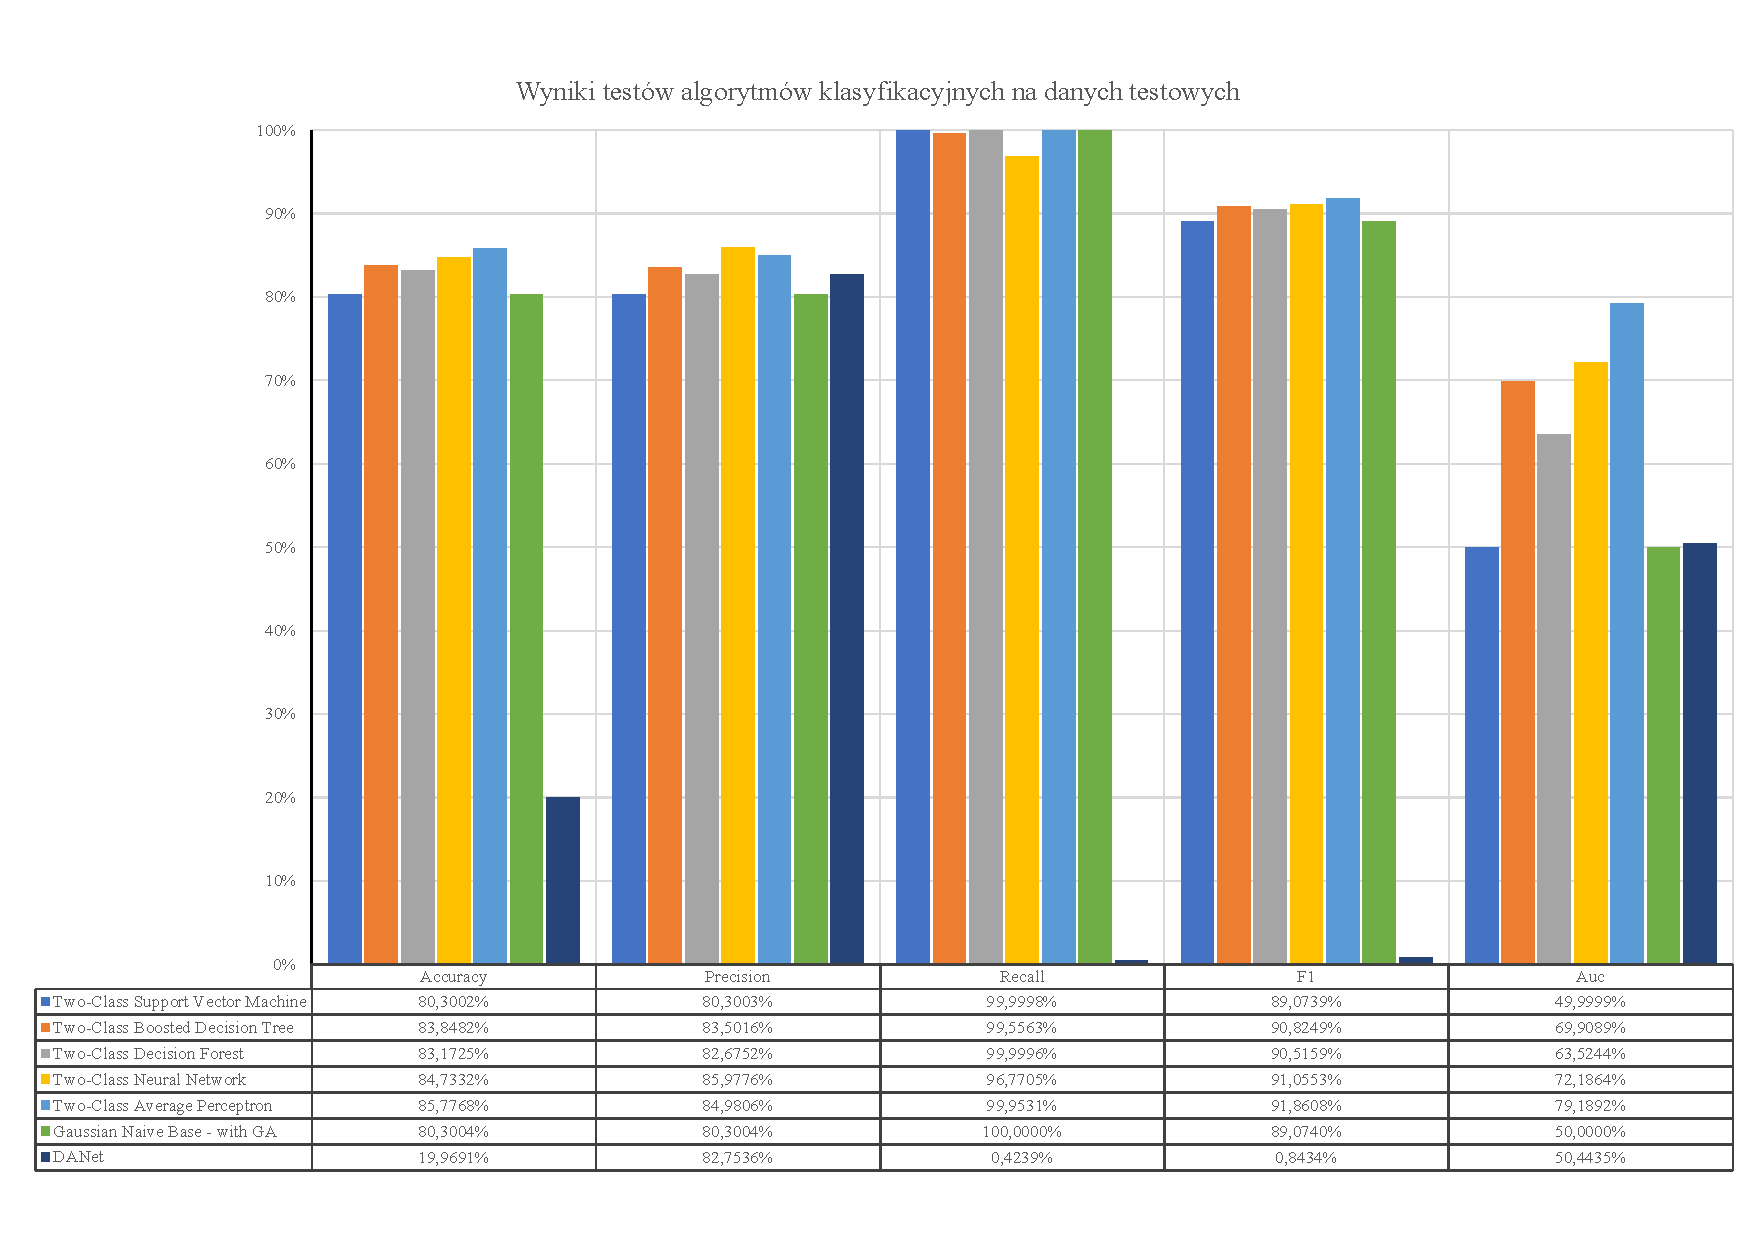
\includegraphics[height=0.8\textwidth]{images/predict_result}
        \captionsource{Wyniki testów algorytmów klasyfikacyjnych na danych testowych}{Opracowanie własne}
        \label{fig:predict-result}
    \end{figure}
    \vfill
\end{landscape}

Poniżej zostały przedstawione wyniki zbiorcze dla poszczególnych metryk.\ Dodatkowo przedstawiono również wynik pomiaru treningowego, który w większości przypadków jest wyższy od danych testowych.\ Co prawdopodobnie jest spowodowane różnicą w ilości danych testowych i treningowych.\ Dodatkowo w każdej kolumnie oznaczono kolorem zielonym najwyższy wynik dla danej metryki, a kolorem czerwonym najniższy wynik dla danej metryki.

\subsection{Dopasowanie}
Najlepszy wynik dopasowania dla danych treningowych uzyskał algorytm \textit{Two-Class Average Perceptron}, który poprawnie rozpoznał $85,7768\%$ próbek.\ Najgorszy wynik uzyskał algorytm \textit{DANet} z dopasowaniem rzędu: $19,9691\%$.\ Dla próby treningowej najlepszy wynik uzyskał \textit{Two-Class Boosted Decision Tree} z wynikiem $100,00\%$, a najgorszy \textit{Two-Class Average Perceptron} z wynikiem $97,4502\%$.\ Wyniki dopasowania dla poszczególnych prób zostały przedstawione na \refsource{tabeli}{tab:acc-res} oraz na wykresie \refsource{wykresie}{fig:acc-res}

\begin{table}[H]
    \centering
    \captionsourceb{Wynik dopasowania algorytmów.}{Kolorem zielonym określono najlepszy wynik w kolumnie.\ Kolorem czerwonym określono najgorszy wynik w kolumnie.}{Opracowanie własne}
    \begin{NiceTabular}{|l|r|r|r||r|}[hvlines]
        & \multicolumn{4}{c|}{\textbf{Wynik dopasowania}} \\
        \textbf{Algorytm}                & \textbf{Próba 1}                  & \textbf{Próba 2}                  & \textbf{Próba 3}                  & \textbf{Próba testowa}             \\
        Two-Class Support Vector Machine & $80,3002\%$                       & $80,3002\%$                       & $80,3002\%$                       & $99,9167\%$                        \\
        Two-Class Boosted Decision Tree  & $83,8482\%$                       & $83,8482\%$                       & $83,8482\%$                       & \cellcolor{lightgreen}$100,0000\%$ \\
        Two-Class Decision Forest        & $83,1725\%$                       & $83,1725\%$                       & $83,1725\%$                       & $99,9960\%$                        \\
        Two-Class Neural Network         & $84,7332\%$                       & $84,7332\%$                       & $84,7332\%$                       & $99,2682\%$                        \\
        Two-Class Average Perceptron     & \cellcolor{lightgreen}$85,7768\%$ & \cellcolor{lightgreen}$85,7768\%$      & \cellcolor{lightgreen}$85,7768\%$       & \cellcolor{lightred}$97,4502\%$             \\
        Gaussian Naive Base - with GA    & $80,3004\%$                       & $80,3004\%$                       & $80,3004\%$                       & $98,8013\%$                        \\
        DANet                            & \cellcolor{lightred}$19,9691\%$   & \cellcolor{lightred}$19,7899\%$   & \cellcolor{lightred}$19,7899\%$      & $99,9823\%$            \\
    \end{NiceTabular}
    \label{tab:acc-res}
\end{table}

\begin{figure}[H]
    \centering
    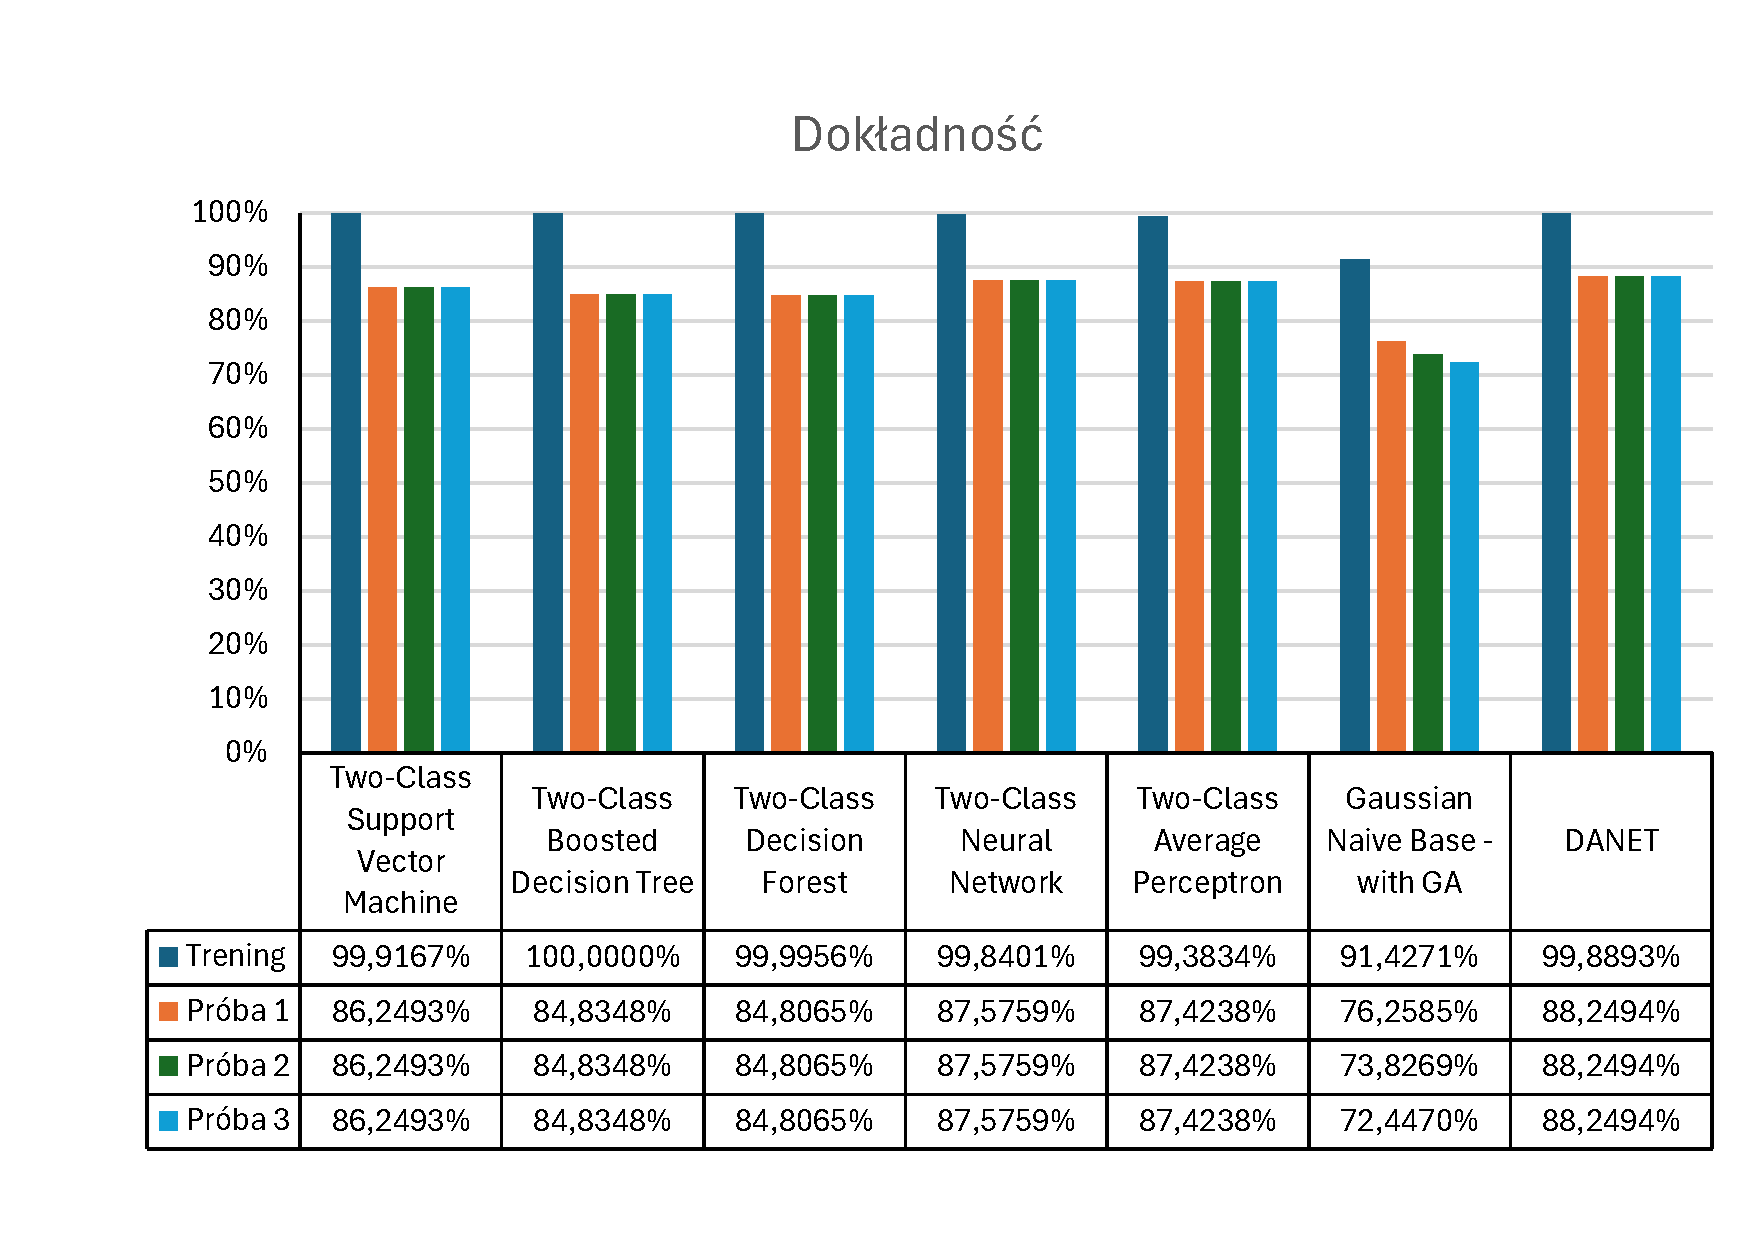
\includegraphics[width=\textwidth]{images/acc-res}
    \captionsource{Dokładność algorytmów}{Opracowanie własne}
    \label{fig:acc-res}
\end{figure}

\subsection{Precyzja}
Najlepszy wynik precyzji uzyskał algorytm ''\textit{Two-Class Neural Network}'' ($85,9776\%$) co oznacza, że najlepiej poradził sobie z dopasowaniem ruchu klasy ''\textbf{1}''. Najsłabszy wynik uzyskał ''\textit{Two-Class Support Vector Machine}'' ($80,3003\%$). GAGNB uzyskał $80,3004\%$ precyzji. Wyniki są opisane w \refsource{tabeli}{tab:acc-prec} oraz na \refsource{wykresie}{fig:acc-prec}.

\begin{table}[H]
    \centering
    \captionsourceb{Wynik precyzji algorytmów.}{Kolorem zielonym określono najlepszy wynik w kolumnie.\ Kolorem czerwonym określono najgorszy wynik w kolumnie.}{Opracowanie własne}
    \begin{NiceTabular}{|l|r|r|r||r|}[hvlines]
        \hline
        & \multicolumn{4}{c|}{\textbf{Wynik precyzji}} \\
        \textbf{Algorytm}                & \textbf{Próba 1}                  & \textbf{Próba 2}                  & \textbf{Próba 3}                  & \textbf{Próba testowa}             \\
        Two-Class Support Vector Machine & \cellcolor{lightred}$80,3003\%$   & \cellcolor{lightred}$80,3003\%$   & \cellcolor{lightred}$80,3003\%$   & $99,8742\%$            \\
        Two-Class Boosted Decision Tree  & $83,5016\%$                       & $83,5016\%$                       & $83,5016\%$                       & \cellcolor{lightgreen}$100,0000\%$ \\
        Two-Class Decision Forest        & $82,6752\%$                       & $82,6752\%$                       & $82,6752\%$                       & $99,9908\%$                        \\
        Two-Class Neural Network         & \cellcolor{lightgreen}$85,9776\%$ & \cellcolor{lightgreen}$85,9776\%$ & \cellcolor{lightgreen}$85,9776\%$ & $99,8972\%$            \\
        Two-Class Average Perceptron     & $84,9806\%$                       & $84,9806\%$                       & $84,9806\%$                       & \cellcolor{lightred}$94,5000\%$    \\
        Gaussian Naive Base - with GA    & $85,7768\%$                       & $80,3004\%$                       & $80,3004\%$                       & $99,8531\%$                        \\
        DANet                            & $82,7536\%$                       & $85,9516\%$                       & $85,9516\%$                       & $99,9887\%$                        \\
    \end{NiceTabular}
    \label{tab:acc-prec}
\end{table}

\begin{figure}[H]
    \centering
    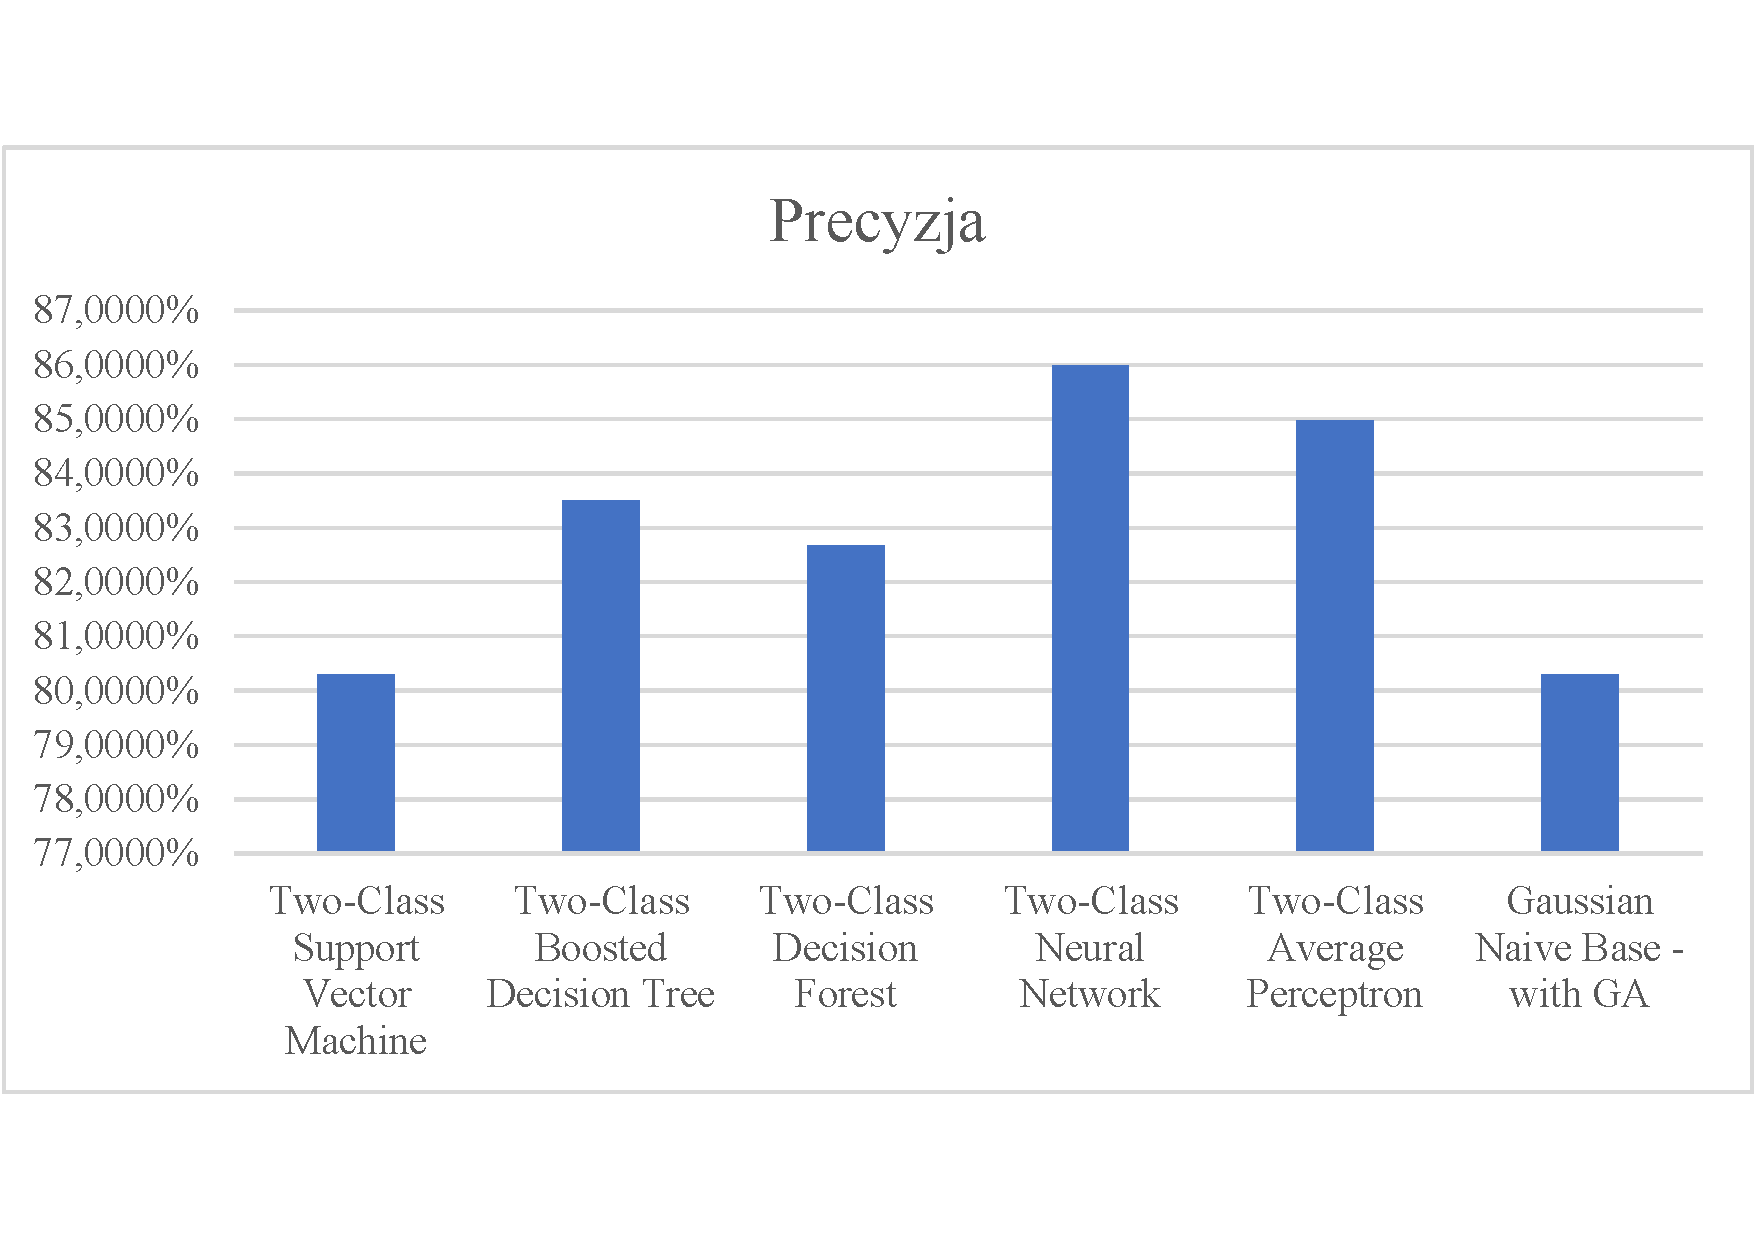
\includegraphics[width=\textwidth]{images/prec-res}
    \captionsource{Precyzja algorytmów}{Opracowanie własne}
    \label{fig:acc-prec}
\end{figure}

\subsection{Czułośc}
Wszystkie wpisy klasy ''\textbf{1}'' zostały poprawnie sklasyfikowane przez algorytm ''\textit{Gaussian Naive Base - with GA}'' ($100\%$), najsłabiej poradził sobie ''\textit{Two-Class Neural Network}'' ($96,7705\%$). Wartości zostały przedstawione w \refsource{tabeli}{tab:rec-res} oraz na \refsource{wykresie}{fig:rec-res}.

\begin{table}[H]
    \centering
    \captionsourceb{Wynik czułości algorytmów.}{Kolorem zielonym określono najlepszy wynik w kolumnie.\ Kolorem czerwonym określono najgorszy wynik w kolumnie.}{Opracowanie własne}
    \begin{NiceTabular}{|l|r|r|r||r|}[hvlines]

        & \multicolumn{4}{c|}{\textbf{Wynik czułości}} \\
        \textbf{Algorytm}                & \textbf{Próba 1}                   & \textbf{Próba 2}                   & \textbf{Próba 3}                   & \textbf{Próba testowa}             \\
        Two-Class Support Vector Machine & $99,9998\%$                        & $99,9998\%$                        & $99,9998\%$                        & $99,9335\%$                        \\
        Two-Class Boosted Decision Tree  & $99,5563\%$                        & $99,5563\%$                        & $99,5563\%$                        & \cellcolor{lightgreen}$100,0000\%$ \\
        Two-Class Decision Forest        & $99,9996\%$                        & $99,9996\%$                        & $99,9996\%$                        & \cellcolor{lightgreen}$100,0000\%$ \\
        Two-Class Neural Network         & $96,7705\%$                        & $96,7705\%$                        & $96,7705\%$                        & $98,4107\%$                        \\
        Two-Class Average Perceptron     & $99,9531\%$                        & $99,9531\%$                        & $99,9531\%$                        & $99,9253\%$                        \\
        Gaussian Naive Base - with GA    & \cellcolor{lightgreen}$100,0000\%$ & \cellcolor{lightgreen}$100,0000\%$ & \cellcolor{lightgreen}$100,0000\%$ & \cellcolor{lightred}$97,3741\%$            \\
        DANet                            & \cellcolor{lightred}$0,4239\%$     & \cellcolor{lightred}$0,1343\%$     & \cellcolor{lightred}$0,1343\%$     & $99,9703\%$            \\
    \end{NiceTabular}
    \label{tab:acc-rec}
\end{table}

\begin{figure}[H]
    \centering
    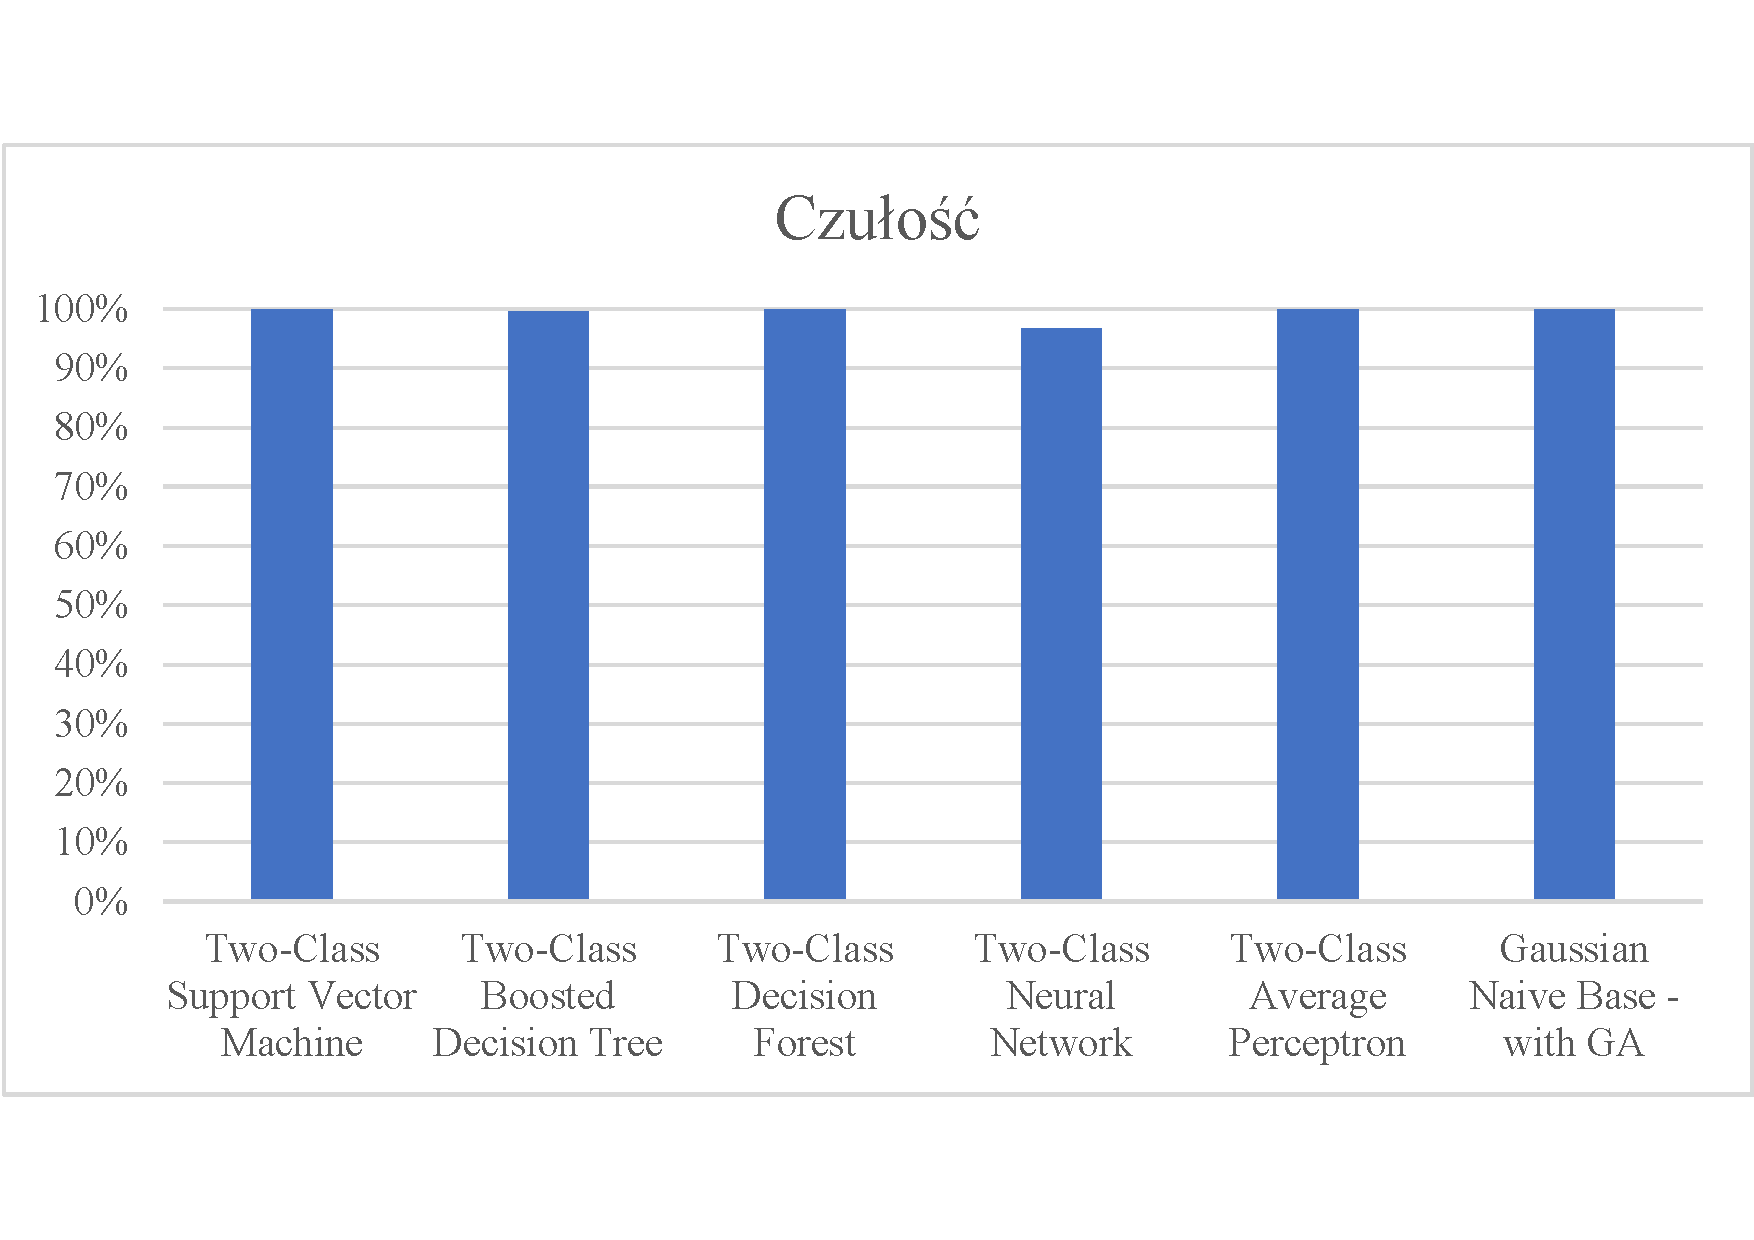
\includegraphics[width=\textwidth]{images/rec-res}
    \captionsource{Czułość algorytmów}{Opracowanie własne}
    \label{fig:rec-res}
\end{figure}

\subsection{F1}
Największą wartość F1 uzyskał ''\textit{Two-Class Average Perceptron}'' ($91,8608\%$). Najmniejszą uzyskał ''\textit{Two-Class Support Vector Machine}'' ($89,0739\%$). GAGNB w tym teście uzyskał $89,0740\%$. Wyniki zostały przedstawione w \refsource{tabeli}{tab:acc-f1} oraz na \refsource{wykresie}{fig:f1-res}.

\begin{table}[H]
    \centering
    \captionsourceb{Wynik F1 algorytmów.}{Kolorem zielonym określono najlepszy wynik w kolumnie.\ Kolorem czerwonym określono najgorszy wynik w kolumnie.}{Opracowanie własne}
    \begin{NiceTabular}{|l|r|r|r||r|}[hvlines]

        & \multicolumn{4}{c|}{\textbf{Wynik F1}} \\
        \textbf{Algorytm}                & \textbf{Próba 1}                  & \textbf{Próba 2}                  & \textbf{Próba 3}                  & \textbf{Próba testowa}             \\
        Two-Class Support Vector Machine & $89,0739\%$                       & $89,0739\%$                       & $89,0739\%$                       & $99,9038\%$                        \\
        Two-Class Boosted Decision Tree  & $90,8249\%$                       & $90,8249\%$                       & $90,8249\%$                       & \cellcolor{lightgreen}$100,0000\%$ \\
        Two-Class Decision Forest        & $90,5159\%$                       & $90,5159\%$                       & $90,5159\%$                       & $99,9954\%$                        \\
        Two-Class Neural Network         & $91,0553\%$                       & $91,0553\%$                       & $91,0553\%$                       & $99,1484\%$                        \\
        Two-Class Average Perceptron     & \cellcolor{lightgreen}$91,8608\%$ & \cellcolor{lightgreen}$91,8608\%$ & \cellcolor{lightgreen}$91,8608\%$ & \cellcolor{lightred}$97,1370\%$            \\
        Gaussian Naive Base - with GA    & $89,0740\%$                       & $89,0740\%$                       & $89,0740\%$                       & $98,5980\%$                        \\
        DANet                            & \cellcolor{lightred}$0,8434\%$    & \cellcolor{lightred}$0,2682\%$    & \cellcolor{lightred}$0,2682\%$    & $99,9795\%$            \\
    \end{NiceTabular}
    \label{tab:acc-f1}
\end{table}

\begin{figure}[H]
    \centering
    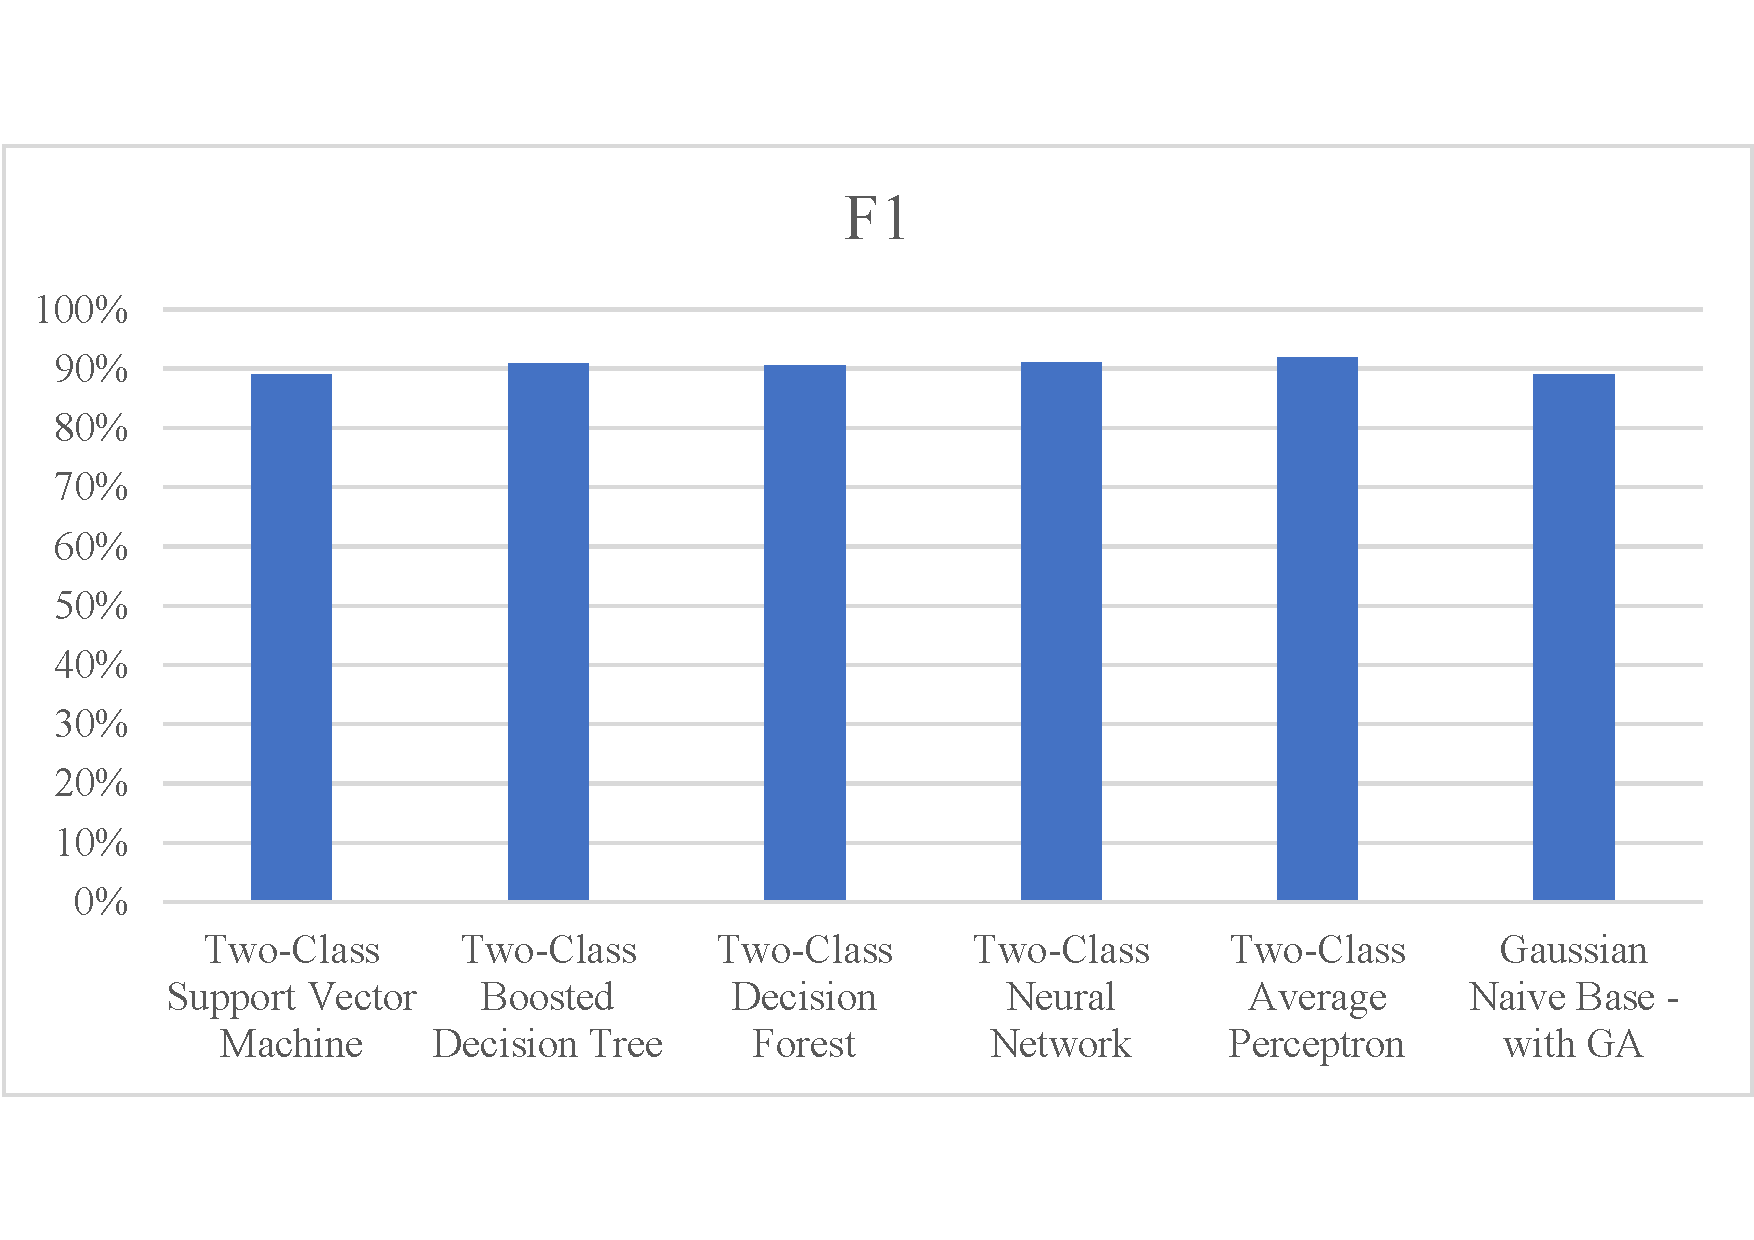
\includegraphics[width=\textwidth]{images/f1-res}
    \captionsource{F1 algorytmów}{Opracowanie własne}
    \label{fig:f1-res}
\end{figure}

\subsection{AUC}
Analizując wynik AUC, można zauważyć, że najlepsza sprawność również uzyskał algorytm ''\textit{Two-Class Average Perceptron}'' ($79,1292\%$). Najgorszy algorytm to znów algorytm wykorzystujący SVM ($49,9999\%$), wynik wskazał na to, że algorytm ten miał niższą sprawność niż próba losowa. W tym teście sprawność algorytmu GAGNB wyniosła $50\%$. Wyniki przedstawiono w \refsource{tabeli}{tab:acc-auc} oraz na \refsource{wykresie}{fig:auc-res}.

\begin{table}[H]
    \centering
    \captionsourceb{Wynik AUC algorytmów.}{Kolorem zielonym określono najlepszy wynik w kolumnie.\ Kolorem czerwonym określono najgorszy wynik w kolumnie.}{Opracowanie własne}
    \begin{NiceTabular}{|l|r|r|r||r|}[hvlines]

        & \multicolumn{4}{c|}{\textbf{Wynik AUC}} \\
        \textbf{Algorytm}                & \textbf{Próba 1}                  & \textbf{Próba 2}                  & \textbf{Próba 3}                  & \textbf{Próba testowa} \\
        Two-Class Support Vector Machine & \cellcolor{lightred}$49,9999\%$   & \cellcolor{lightred}$49,9999\%$ & \cellcolor{lightred}$49,9999\%$     & $99,9974\%$            \\
        Two-Class Boosted Decision Tree  & $69,9089\%$                       & $69,9089\%$                       & $69,9089\%$                       & \cellcolor{lightgreen}$100,0000\%$           \\
        Two-Class Decision Forest        & $63,5244\%$                       & $63,5244\%$                       & $63,5244\%$                       & \cellcolor{lightgreen}$100,0000\%$           \\
        Two-Class Neural Network         & $72,1864\%$                       & $72,1864\%$                       & $72,1864\%$                       & $99,9867\%$            \\
        Two-Class Average Perceptron     & \cellcolor{lightgreen}$79,1892\%$ & \cellcolor{lightgreen}$79,1892\%$ & \cellcolor{lightgreen}$79,1892\%$ & $99,9808\%$            \\
        Gaussian Naive Base - with GA    & $50,0000\%$                       & $50,0000\%$                       & $50,0000\%$                       & \cellcolor{lightred}$99,9437\%$            \\
        DANet                            & $50,4435\%$                       & $76,7282\%$                       & $76,7282\%$                       & $99,9993\%$            \\
    \end{NiceTabular}
    \label{tab:acc-auc}
\end{table}

\begin{figure}[H]
    \centering
    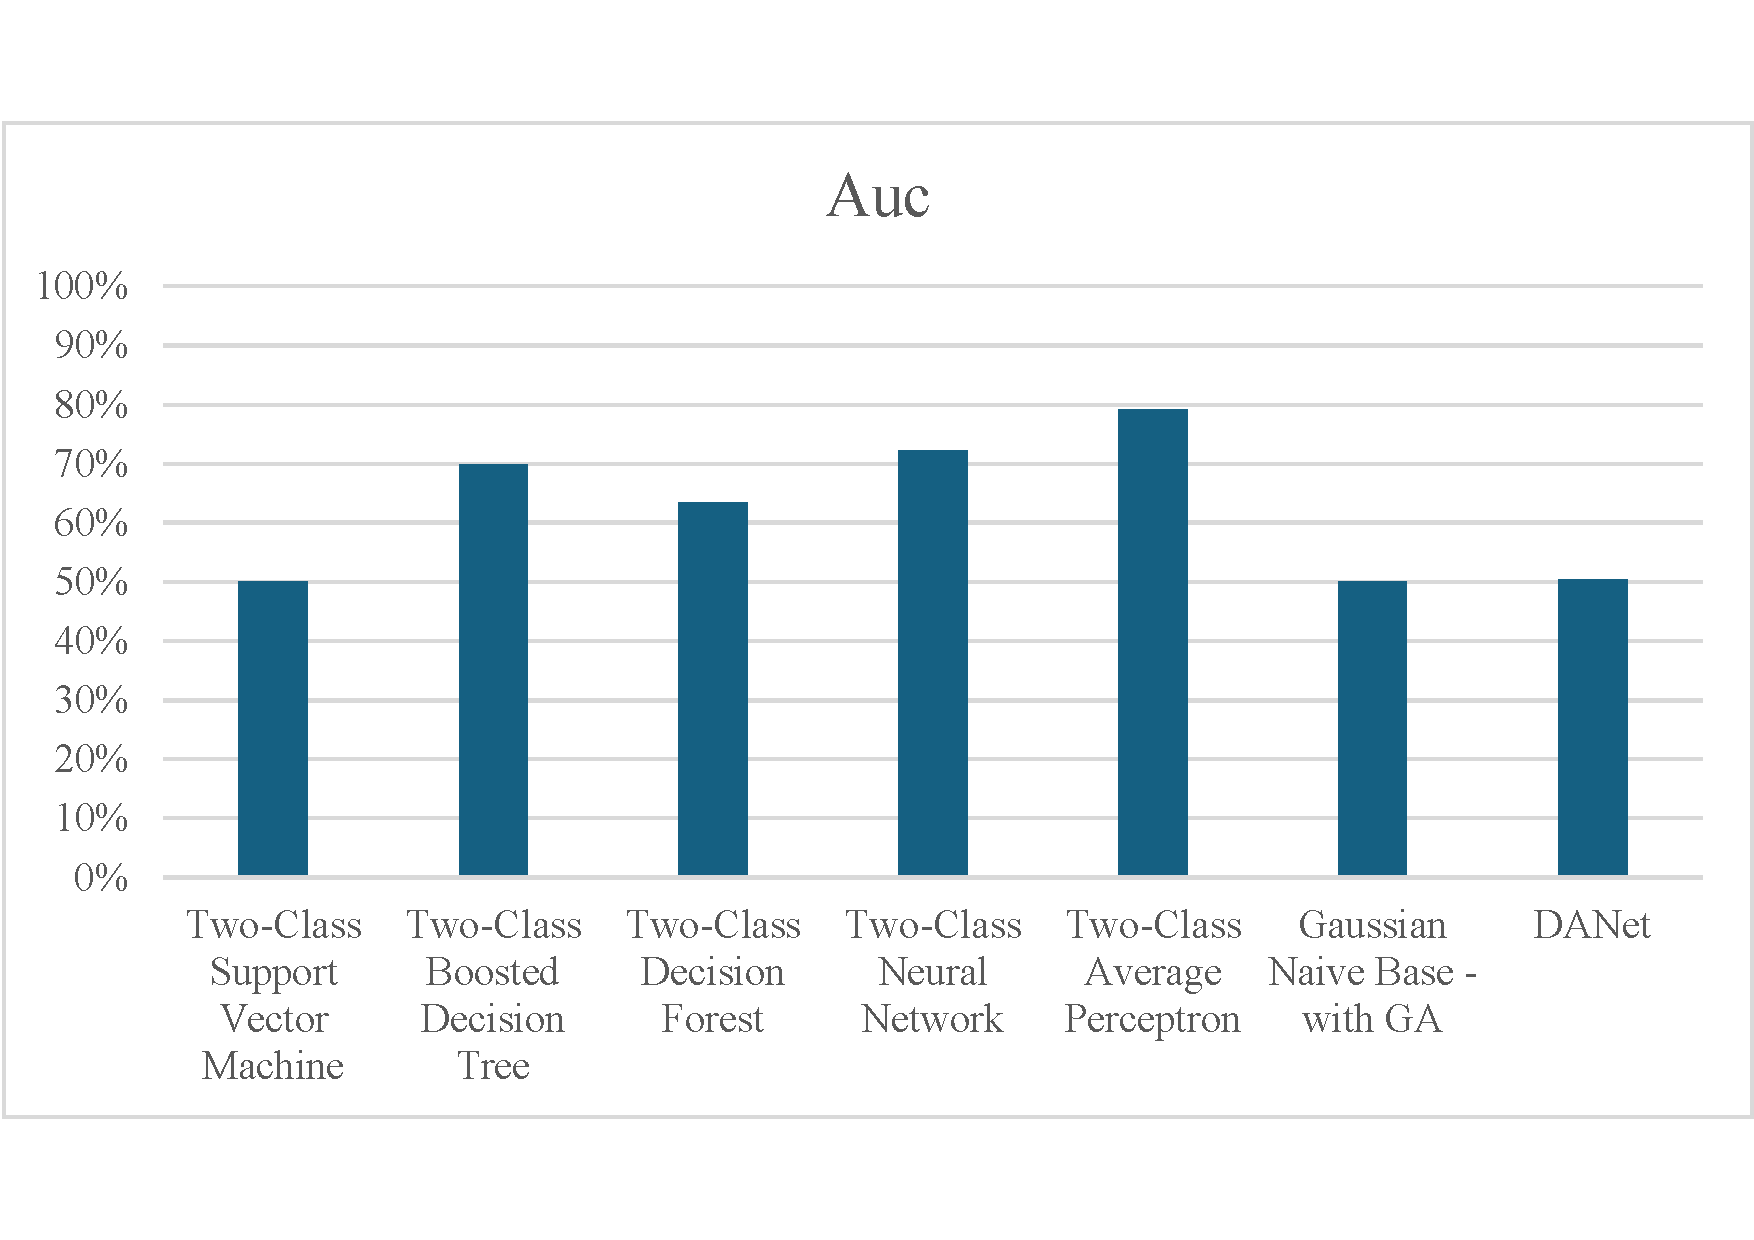
\includegraphics[width=\textwidth]{images/auc-res}
    \captionsource{AUC algorytmów}{Opracowanie własne}
    \label{fig:auc-res}
\end{figure}


\section{Analiza wyników}

Przedział ufności dla dokładności algorytmów wyniósł $17,7218$ dla $\alpha = 0.05$.\ Biorąc pod uwagę ten fakt można stwierdzić, że dokładność algorytmu DANet jest poniżej dolnej granicy.\ Dolna granica przedziału ufności wynosi $56,2925\%$, zaś DANet uzyskał $19,9691\%$ oraz poprawnie zaklasyfikował jedynie $565273$ wpisów.


\section{Wnioski}

Microsoft Wyszedł na przeciw potrzebom użytkowników dlatego przygotował zestaw prekonfigurowanych algorytmów klasyfikacyjnych, dzięki czemu możliwości narzędzia Azure ML pozwalają na odpowiadanie na konkretne potrzeby przy relatywnie niewielkich kosztach. Jednakże to nie oznacza, że tworzenie autorskich rozwiązań mija się z celem. Jak ukazano na \refsource{wykresie}{fig:predict-result} autorskie rozwiązania również mają rację bytu. Wykorzystanie połączenia algorytmu genetycznego i klasyfikatora naiwnego Bayesa z rozkładem normalnym pozwala na uzyskanie zbliżonych wyników co algorytmu utworzone przez giganta technologicznego. Różnica około 5 punktó procentywych między najlepszym algorytmem a algorytmem GAGNB ukazuje niewielką różnicę w jakości algorytmu. Dodatkowo wciąż trudno korzysta się z rozwiązań takich jak DANet, któe są nieprzetestowe na różnorakich zbiorach lecz na tych wcześniej specjalnie spreparowanych.
\\ \\
Dodatkowo korzystanie z tego typu prostych rozwiązań autorskich pozwala na prototypownie rozwiązań biznesowych opartych o klasyfikację danych. Samo wykorzystanie algorytmu genetycznego z algorytmem GNB umożliwia skupienie się na tworzenie ugólnego rozwiązania bez wcześniejszej znajomości zbioru oraz korzystając z programów lokalnie nie ponosząc kosztów wykorzystania platformy chmurowej. Kolejnym atutem utworzonego przez autora rozwiązania jest zmniejszenie kosztów lokalnego użytkowania poprzez zmniejszenie wymiarowości zbioru danych do klasyfikacji poprzez wykorzystanie jedynei wytypowanych kolumn.
\\ \\
Doświadczenie to ukazuje, że wciąż należy próbować tworzyć wydajniejsze i dokładniejsze rozwiązania, lecz nie zaprzecza faktu iż rozwiązania ogólnie dostępne są na bardzo wysokim poziomie. Uzyskano dokładność z zakresu $[80\%, 85\%]$ przy czym plik testowy był 12 krotnie większy od pliku treningowego.

